\documentclass[9pt]{beamer}
\usepackage{beamerthemeshadow}
\usepackage{amsmath}
%\usepackage{ctex}
\usepackage{float}
\usepackage{graphicx}
\DeclareGraphicsExtensions{.eps,.ps,.jpg,.bmp,.pdf}
\usepackage{cite}
\usepackage{url}

\usetheme{Warsaw}
\linespread{1.1}

\title{Great Again or Stronger Together? Sentiment Analysis About Book Reviews on Amazon}
\author{Jiabao Wu\thanks{Central University of Finance and Economics}, Siyan Li\footnotemark[1] \\ \footnotesize lisiyan6315@foxmail.com}
\date{\today}

\begin{document}

\begin{frame}
\titlepage
\end{frame}

\begin{frame}
\frametitle{Background}
During the presidential election in the year of 2016, Donald Trump, a fruitful writer, businessman and talk show host, swept adverse remarks away and flushed to the top against his rival, Hillary Clinton, as the 45th American president.

In this election, both of the main candidates have published a book to elaborate their ideas for political propaganda. Donald Trump published \textit{Great Again: How to Fix Our Crippled America}(\textit{GreatAgain} for short) in July 12, 2016 while Hillary Clinton published \textit{Stronger Together: A Blueprint for America's Future}(\textit{Blueprint} for short) in Sep 6, 2016. These two books are both wildly read, commented and frequently referred in their speeches. In another word, there are many interesting and valuable messages implied in book reviews.
\end{frame}

\begin{frame}
\frametitle{Objectives}
Given the messages above, we are aimed at data mining towards book reviews on bestsellers by Trump and Hillary. Our analysis focus on 5 questions listed below.
\begin{itemize}
	\item How do book readers level Trump and Hillary's bestsellers?
	\item Which words are mainly used in book reviews on their bestsellers?
	\item What's the main difference in book reviews between Trump and Hillary?
	\item How did book readers feel when they give comments?
	\item What differs mostly between positive comments and negative ones?
 \end{itemize}
\end{frame}

\begin{frame}
\frametitle{Procedures}
The following parts are constructed as follows:
\begin{itemize}
	\item Collecting book reviews
	\item Data cleaning
	\item Drawing word clouds
	\item Extracting words with high distinction between two books
	\item Sentiment analysis by VADER between two books
	\item Extracting words with high distinction between positive and negative reviews
	\item Sentiment analysis by VADER between positive and negative reviews
\end{itemize}
\end{frame}

\begin{frame}
\frametitle{Collecting book reviews}
Our research collected book reviews of both candidates' bestsellers on Amazon during US presidential election. \textit{GreatAgain} was published on 12th July, 2016. \textit{Blueprint} was published on 6th September, 2016. We collected all book reviews untill the election day(8th Nonvember, 2016). An Example of book review is shown below.
\begin{figure}[H]
	\centering
	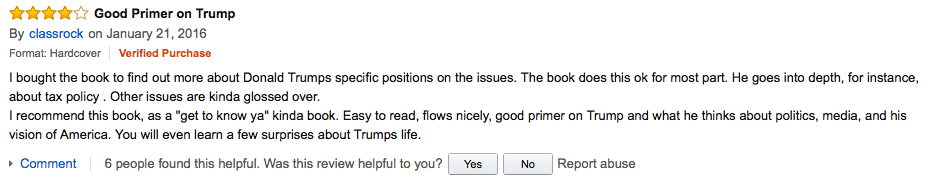
\includegraphics[width=250pt]{amazon_review.png}
	\caption{Book review example on Amazon}
\end{figure}
As is showed in figure above, our data contains 6 sects. Book reviews were cleaned by a filter capable of extracting the number of stars, dates and contexts from Amazon's book reviews. As for other parts, names and formats were excluded for the sake of privacy conservation, and titles were omitted because of duplicate content and the excessive quantity of missing values.
\end{frame}

\begin{frame}
\frametitle{Collecting book reviews}
\begin{table}[H]
	\centering
	\begin{tabular}{ccccc}
		\hline
		Title & NumberOfReviews & MeanOfRates & HighRates & LowRates \\
		\hline
		GreatAgain & 1342 & 4.34 & 1170(87.4\%) & 169(12.6\%) \\
		Blueprint & 2556 & 1.45 & 295(11.5\%) & 2261(88.5\%) \\
		\hline
	\end{tabular}
\end{table}
\begin{figure}[H]
	\centering
	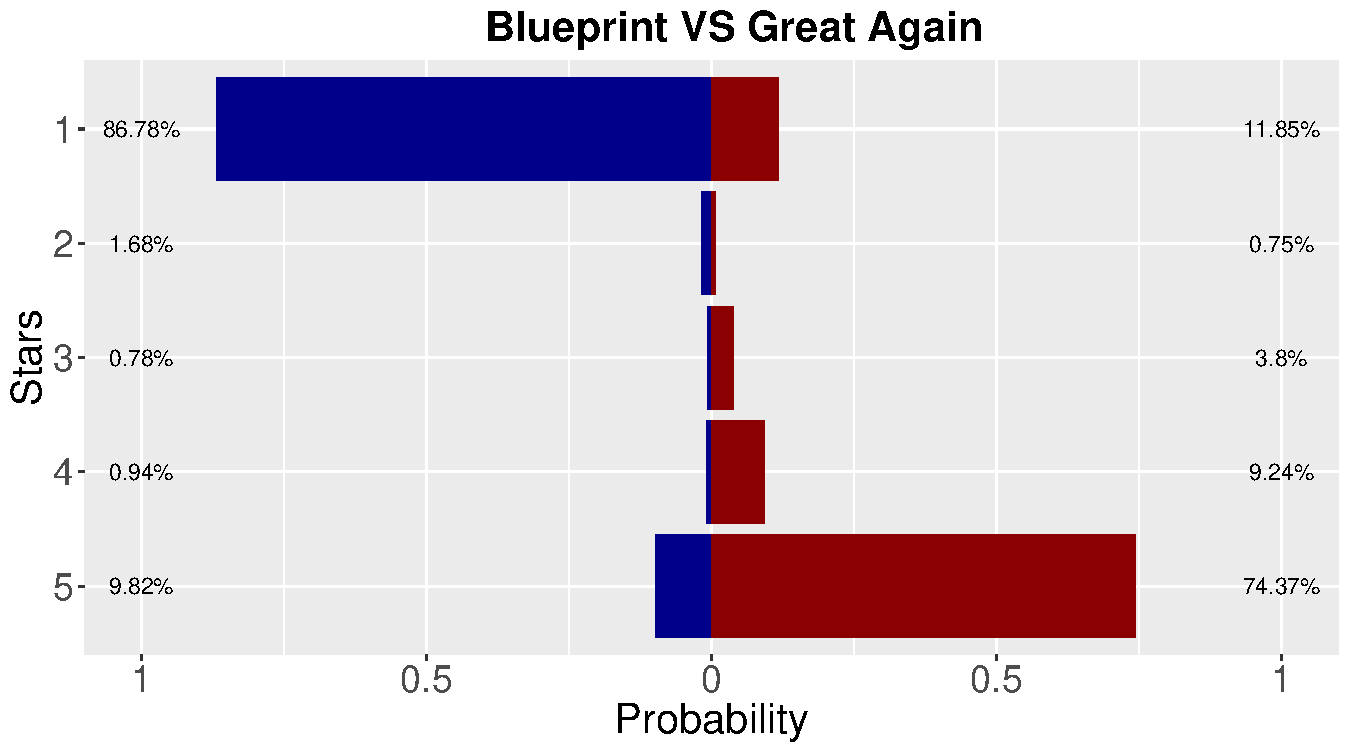
\includegraphics[width=250pt]{评分比较_bar.pdf}
\end{figure}
\end{frame}

\begin{frame}
\frametitle{Data cleaning}
\begin{itemize}
	\item Tokenization
	\item Capitalization conversion
	\item Noise cleaning(punctuations, numbers and weblinks)
	\item Stopwords removal
	\item Remove following four words: 'book', 'read', 'amazon', 'review'
	\item Stemming and lemmatization
\end{itemize}
\end{frame}

\begin{frame}
\frametitle{Drawing word clouds}
\begin{figure}[H]
	\centering
	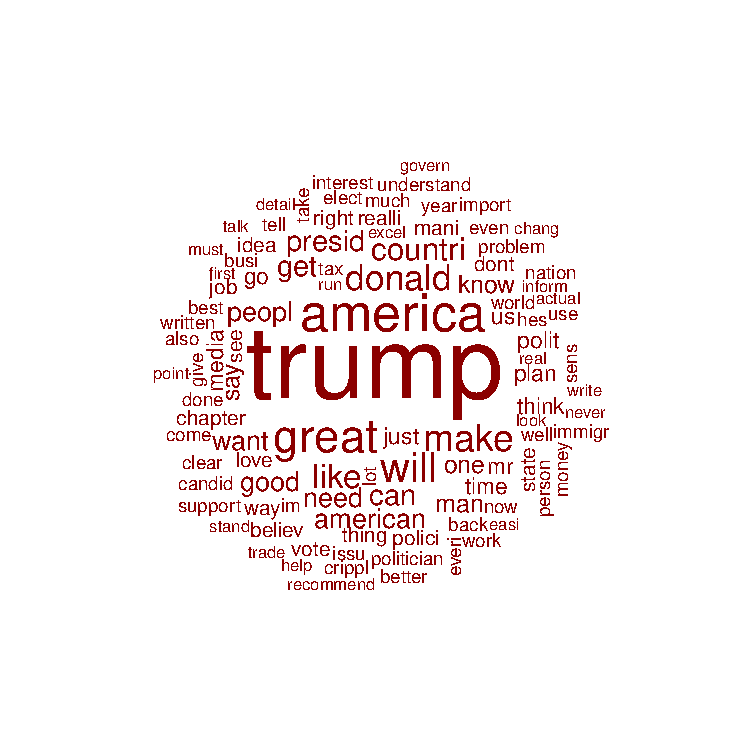
\includegraphics[width=150pt]{great_词云.pdf}
	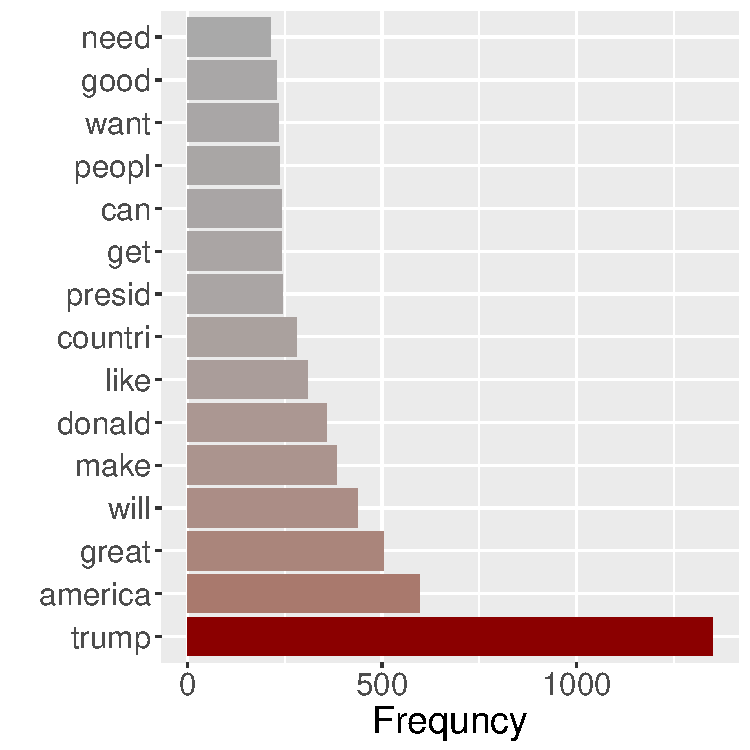
\includegraphics[width=150pt,height=150pt]{great_bar.pdf}
	\caption{Book review of \textit{GreatAgain}}
\end{figure}
The unique words in comments on Trump are 'Great', 'America', 'country', 'preside' and 'good', which are all positive words and closely related to country's future.
\end{frame}

\begin{frame}
\frametitle{Drawing word clouds}
\begin{figure}[H]
	\centering
	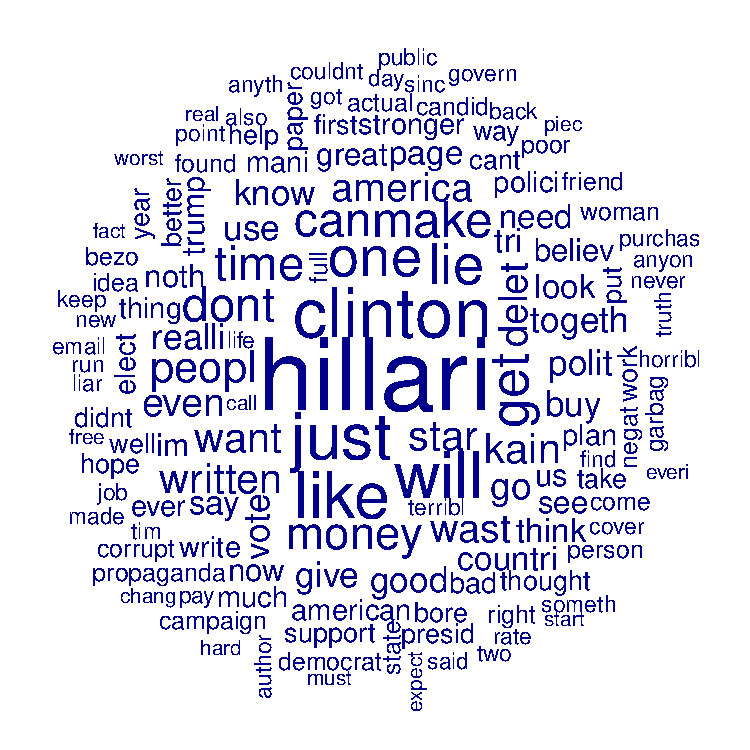
\includegraphics[width=150pt]{blue_词云.pdf}
	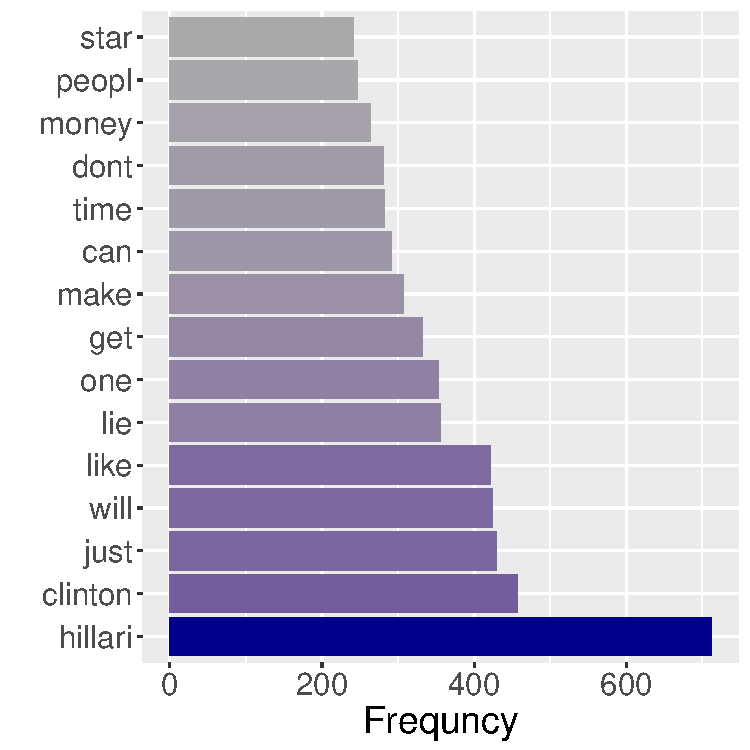
\includegraphics[width=150pt,height=150pt]{blue_bar.pdf}
	\caption{Book review of \textit{Blueprint}}
\end{figure}
The unique words in comments on Hillary are 'just', 'lie', 'money' and 'dont', which are mostly negative words, attacking Hillary's political affairs.
\end{frame}

\begin{frame}
\frametitle{Extracting words with high distinction between two books}
We consider book reviews as bag-of-words, using word counts as text features and random forest as text classifier in order to classify whether a comment is aimed at Hillary or Trump. The accuracy rate of 10-fold cross validation is 81\%, which means our text features are able to extract main differences between different authors.
\begin{table}[H]
	\centering
	\caption{Accurancy \& Confusion Matrix}
	\begin{tabular}{cccc}
		\hline
		Accurancy: & 0.8843 & & \\
		\hline
		& Truth & GreatAgain & Blueprint \\
		\hline
		Predict & GreatAgain & 220 & 25 \\
		        & Blueprint & 30 & 119 \\
		\hline
	\end{tabular}
\end{table}
\end{frame}

\begin{frame}
\frametitle{Extracting words with high distinction between two books}
\begin{figure}[H]
	\centering
	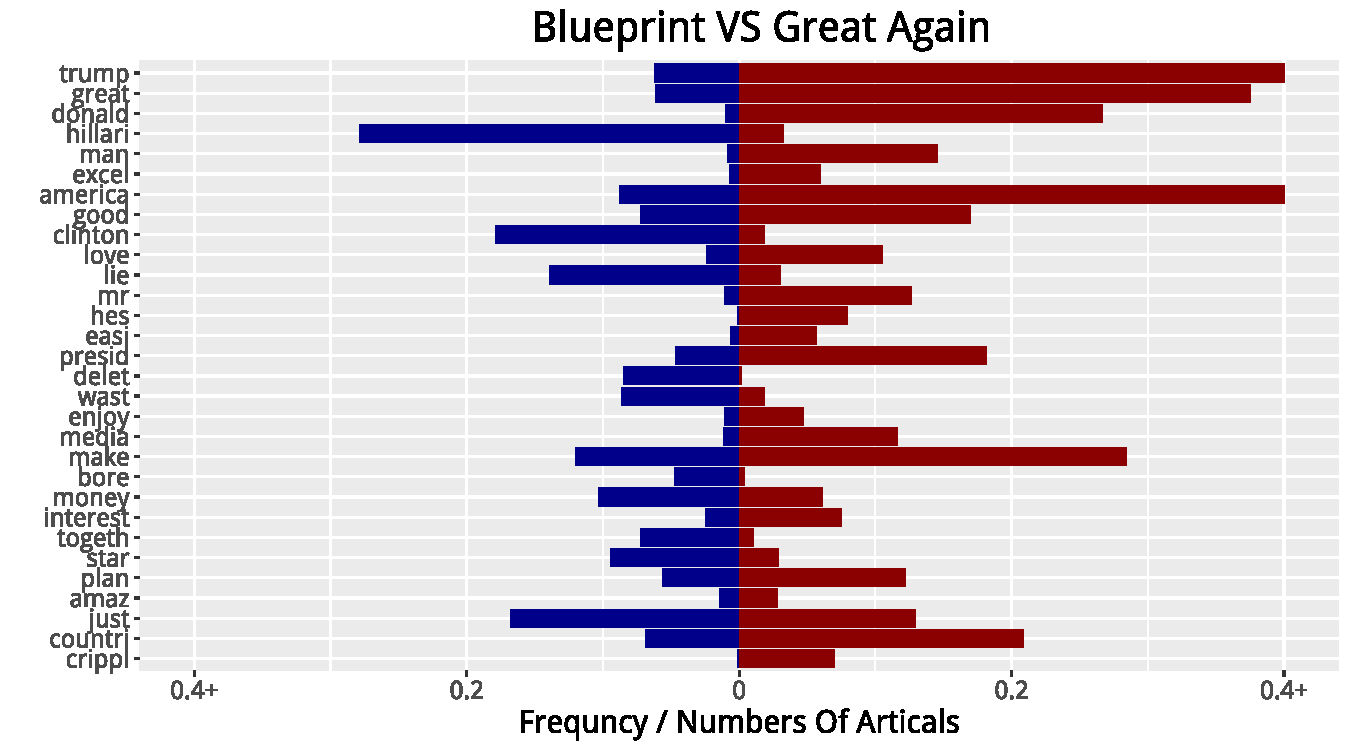
\includegraphics[width=250pt]{bagofwords_bar.pdf}
\end{figure}
\begin{table}[H]
	\centering
	\begin{tabular}{cp{200pt}}
		\hline
		 \textit{GreatAgain} features & trump, great, donald, man, excel, american, good, love, mr,  hes, easi, presid, enjoy, media, make, interest, plan, amaz, countri, crippl \\
		 \hline
		 \textit{Blueprint} features & hillari, clinton, lie, delet, money, wast, bore, togeth, star, just \\
		\hline
	\end{tabular}
\end{table}
\end{frame}

\begin{frame}
\frametitle{Sentiment analysis by VADER between two books}
VADER, or Valence Aware Dictionary for sEntiment Reasoning, is a sentiment analysis toolkit, based on Emotional lexicon. This toolkit is proposed in\"VADER: A Parsimonious Rule-based Model for Sentiment Analysis of Social Media Text\".

When dealing with microblog-like contexts, VADER outperforms eleven other state-of-practice benchmarks, including LIWC, SentiWordNet, and the General Inquirer. VADER uses a combination of qualitative and quantitative methods to build an exotic emotional vocabulary for Internet slang and its algorithm, based on word-of-bag model, about the same as LIWC. However, VADER is far more expert at discovering word-order sensitive relations between terms.
\end{frame}

\begin{frame}
\frametitle{Sentiment analysis by VADER between two books}
We obtain sentimental evaluation of each review by VADER, each review contains degree of positive, negative and neural emotion. We draw kernel density curve of different emotions between different authors. The result is shown below.
\begin{figure}[H]
	\centering
	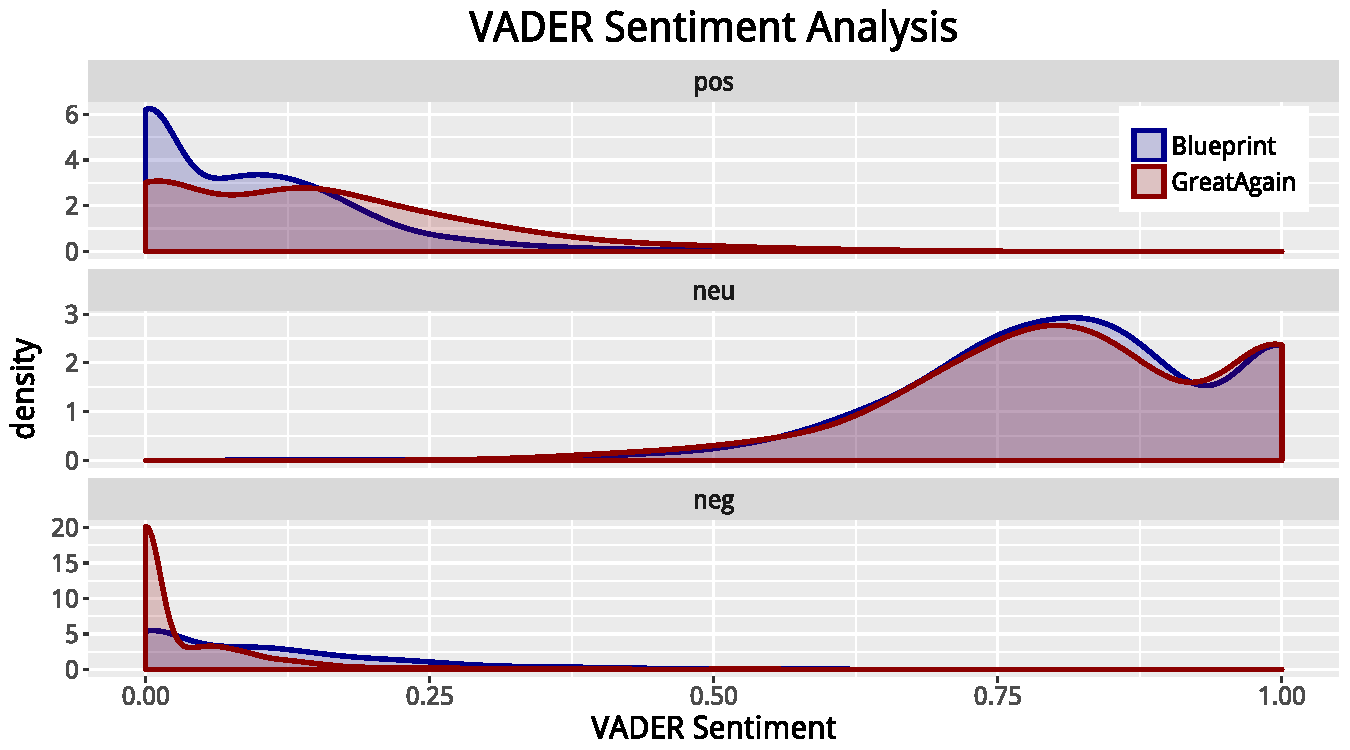
\includegraphics[width=250pt]{vader_density.pdf}
	\caption{Both candidates' reviews are sentimentally neuralized. However, Trump gets more comments with positive emotion and less with neural and negative ones, while Hillary less positive and more negative.}
\end{figure}
\end{frame}

\begin{frame}
\frametitle{Extracting words with high distinction between positive and negative reviews}
In this part we aim at exploring difference between positive and negative reviews. We define positive review as those leveled 4 or more stars, and negative review 3 or less stars. We use the bag-of-word model and random forest to extract words with high distinction between positive and negative reviews.
\end{frame}

\begin{frame}
\frametitle{Extracting words with high distinction between positive and negative reviews}
\begin{figure}[H]
	\centering
	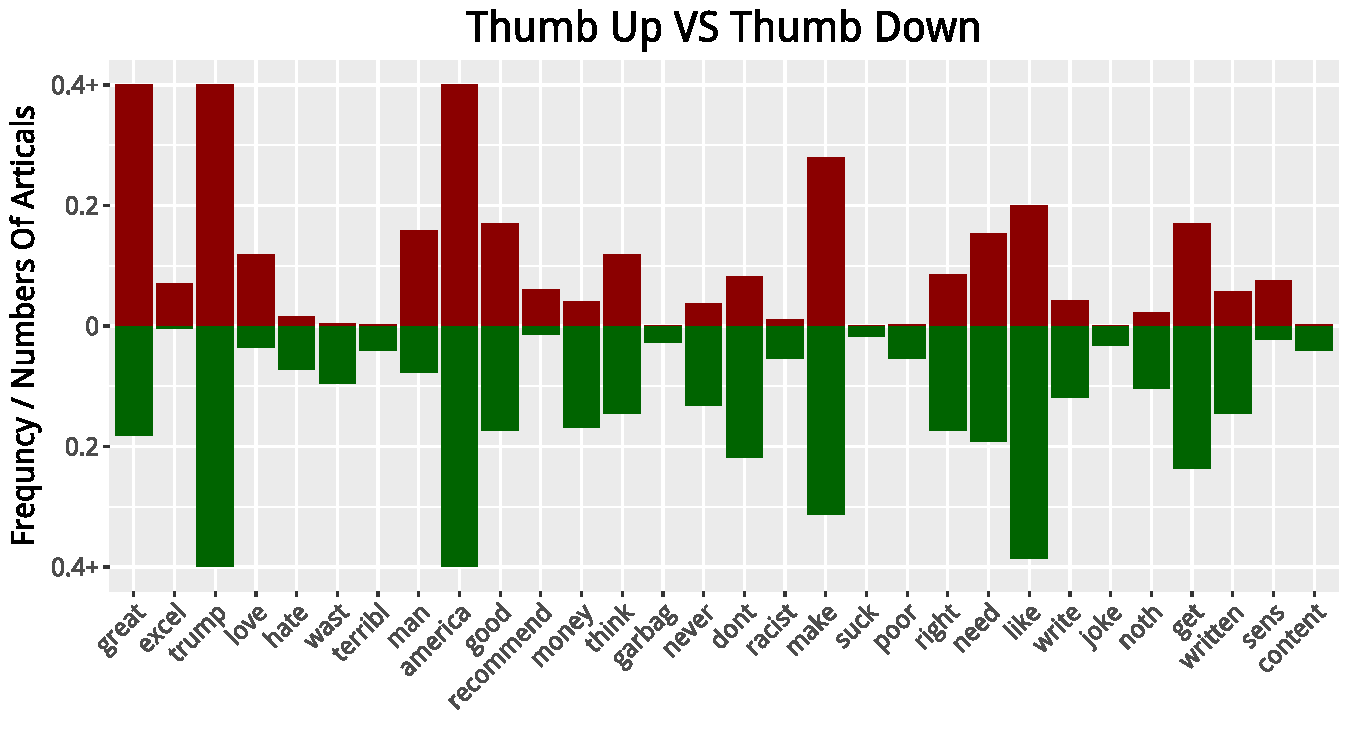
\includegraphics[width=250pt]{bagofwords_great_bar.pdf}
\end{figure}
\begin{table}[H]
	\centering
	\begin{tabular}{cp{200pt}}
		\hline
		 ThumbUp features & great, excel, love, man, good, recommend, sens \\
		 \hline
		 ThumbDown features & hate, wast, terribl, money, think, garbag, never, dont, racist, make, suck, poor, right, need, like, write, joke, noth, get, written, content \\
		\hline
	\end{tabular}
\end{table}
\end{frame}


\begin{frame}
\frametitle{Extracting words with high distinction between positive and negative reviews}
\begin{figure}[H]
	\centering
	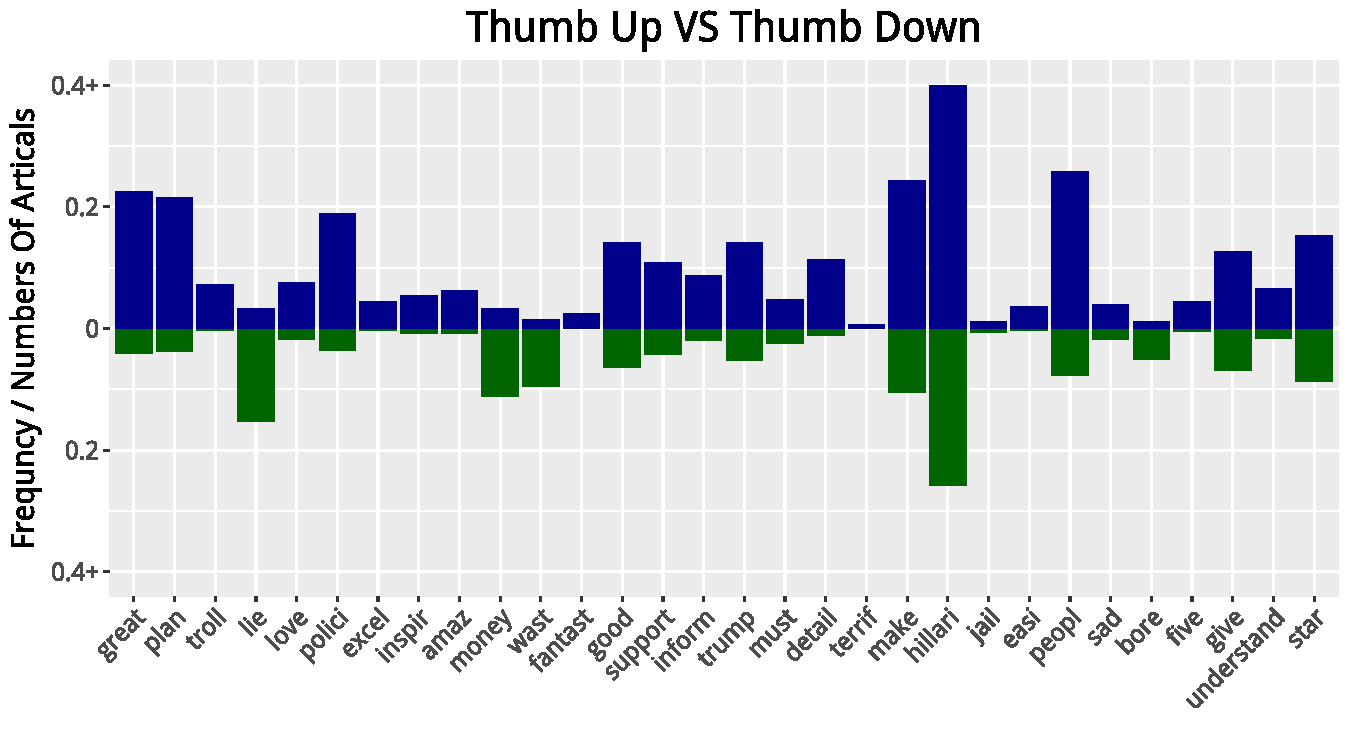
\includegraphics[width=250pt]{bagofwords_blue_bar.pdf}
\end{figure}
\begin{table}[H]
	\centering
	\begin{tabular}{cp{200pt}}
		\hline
		 ThumbUp features & great, plan, troll, love, polici, excel, inspir, amaz, fantast, good, support, inform, trump, must, detail, make, hillari, easi, peopl, sad, five, give, understand, star \\
		 \hline
		 ThumbDown features & lie, money, wast, terrif, jail, bore \\
		\hline
	\end{tabular}
\end{table}
\end{frame}

\begin{frame}
\frametitle{Sentiment analysis by VADER between positive and negative reviews}
\begin{figure}[H]
	\centering
	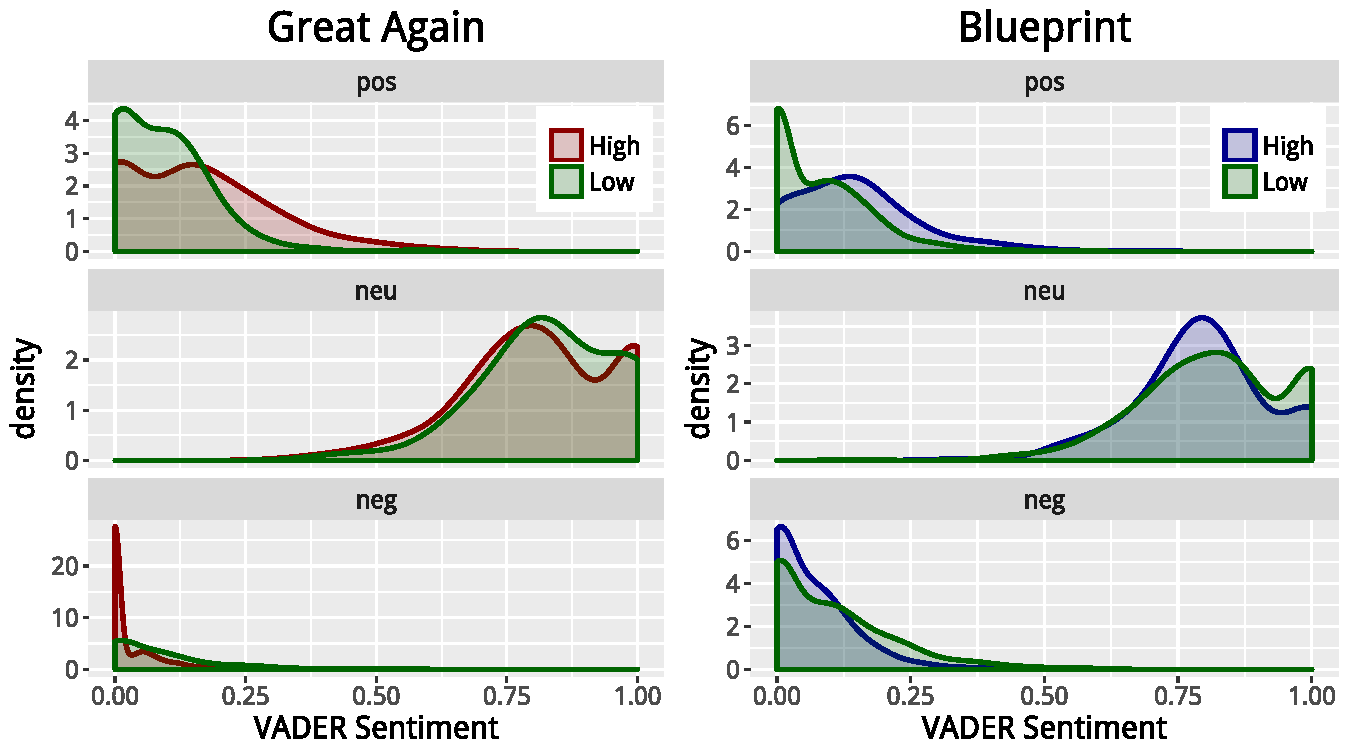
\includegraphics[width=300pt]{vader比较_density.pdf}
	\caption{VADER Sentiment Analysis}
\end{figure}
\end{frame}

\begin{frame}
\frametitle{Conclusion}
\large{\textbf{1.How do book readers level Trump and Hillary's bestsellers?}}

On Amazon, most readers gave Trump's bestseller high rates. On the contrary, most readers gave Hillary's bestseller low rates.

\large{\textbf{2.Which words are mainly used in book reviews on their bestsellers?}}

The unique words in comments on Trump are ’Great’, ’America’, ’country’, ’preside’ and ’good’, most of which are positive words and closely related to country's future. In contrast, the unique words in comments on Hillary are ’just’, ’lie’, ’money’ and ’dont’,
which are mostly negative words, attacking Hillary’s political affairs.
\end{frame}

\begin{frame}
\frametitle{Conclusion}
\large{\textbf{3.What's the main difference in book reviews between Trump and Hillary?}}

Reviews on the Trump's bestseller used more words that reflect positive emotions and nature of leadship, while reviews on Hillary's bestseller use more words which imply conspiracy theory and reflect negative emotions.

\large{\textbf{4.How did book readers feel when they give comments?}}

Compared with the readers of \textit{Blueprint}, the readers of \textit{GreatAgain} used more words to reflect positive emotions, less words to reflect neutral and negative emotions, which shows the readers of \textit{Blueprint} are more exciting than the orthers.

\large{\textbf{5.What differs mostly between positive comments and negative ones?}}
\end{frame}
\end{document}
